% \documentclass[twocolumn]{article}
\documentclass{article}
% \documentclass[useAMS,usenatbib]{mnras}
\usepackage[utf8]{inputenc}

\usepackage{graphicx}% Include figure files
\usepackage{xcolor}
\usepackage{epstopdf}% Allows eps figures
\usepackage{float}% Better image placement
\usepackage{enumerate}

\usepackage{textcomp,gensymb}% Adds general symbols
\usepackage{amsmath, amssymb}% Math symbols and stuff
\usepackage{mathtools}% math things

\usepackage[numbers,sort&compress]{natbib}% Hyperlink References
\usepackage{hyperref}% Hyperlink References

\usepackage{ulem}
\usepackage[capitalise]{cleveref}

\newcommand{\dnp}[1]{\textcolor{cyan}{#1}}


\title{Quick Notes about Machine Learning on Intensity Maps}
\author{Daniel N. Pfeffer}
\date{}

\graphicspath{{images/}}

\begin{document}
% \bibliographystyle{unsrtnat}

	\maketitle

	\begin{abstract}
		The idea of this project is to use machine learning on intensity maps to determine the luminosity function of the underlying halos.
	\end{abstract}

	\section{Intensity Maps Background} \label{sec:IMback}

		Intensity mapping is done by looking at a given emission line.  Whatever is being traced should be emitting this line at any location where the tracer is located.  Having a higher density of the tracer would cause an increased intensity of whatever line is being looked at.  As the light travels to Earth it will get redshifted based on where it was originally emitted.  By looking at a range of frequencies one can get 3D spatial information (maps) about whatever tracer is being looked at.  

		George has code to generate different halo catalogs quickly and has done so to make (as of the time of writing this part) 161 halo catalogs.  Each of these catalogs can be converted into smaller subfields as well as rotated to produce more catalogs.  With another code of George's one can convert these halo catalogs (or regions in them) into intensity maps.  We want lots of intensity maps so that we can do machine learning on the maps to determine the underlying luminosity function.

	\section{Machine Learning Background} \label{sec:MLback}

		I'm feeling lazy right now and don't want to fully flesh this out yet.

		Machine learning can be used for lots of tings if you throw enough data at it.  

		Neural networks are supposed to represent how brains and neurons work.  It is trained for a specific task and each neuron has it's own weights.  This gets very memory intensive for large networks because there can be lots of neurons.  A way around this is to use convolutional neural networks (CNN).  A CNN has filters that convolve with layers of input or neuron output and each layer has the same filter which saves on memory.  A quick Google showed these links that explain CNNs both in depth (http://cs231n.github.io/convolutional-networks/) and at a surface level (https://medium.freecodecamp.org/an-intuitive-guide-to-convolutional-neural-networks-260c2de0a050).

	\section{Intensity Mapping CNN} \label{sec:cnn}

		As of right now the idea is to use a CNN on simulated intensity maps to determine the luminosity function of the underlying halos that made the simulated intensity maps.  George has code to make the halo catalogs and another code to convert the catalogs into intensity maps.  I've made code to split up the catalogs into smaller subfields to match possible experiments.  I also have code that will rotate the halo catalogs before making subfields so that we have more subfields to train out network with.  George's code limlam mocker (llm) (the code that converts catalogs into intensity maps) was modified by me to also give out the luminosity function of the underlying halos.  The llm can also use different underlying halo luminosity relations to generate different maps and luminosity functions.

		As of the basic training right now I am not doing anything to split up the maps into training, validation and test sets.  I'm just seeing the general results of different things right now.

		\subsection{log dN/dL} \label{sec:logValue}
			Originally the CNN was trained on converting an intensity map into \(\log dN/dL\) instead of just \(dN/dL\).  This was done originally to prevent having such a large range of output values could be hard to train.

			As of right now I have a trained network that is 4 layers that trained for 100 epochs of 400 maps apiece.  Each layer is a 3D convolution with kernel size 5 and stride 1 followed by a max pooling 3D of size 2 and stride 2.  The first layer has 32 filters, followed by 64, 128 and 256.  Following the convolutional layers the network is flattened and then has a dense layer with 1000 neurons.  The final layer is another dense layer with a neuron for each point in the luminosity function we want.  Currently I take 50 points of the luminosity function.  The loss function was just the mean square error function.

			\dnp{Should get plots for accuracy and loss as a function of time, but forgot to add that functionality to the CNN when I first ran it}.  The network took under 30 hours to train.  \cref{fig:CNN_4_layer_log,fig:CNN_4_layer_log_ratio,fig:CNN_4_layer_log_ratio_small} show the result of the CNN on some random map.  In all luminosity bins before around \(L = 10^6 L_{sun}\) the CNN luminosity function is within a couple of percent of the underlying one.  After \(L = 10^6 L_{sun}\) the ratio of CNN luminosity function to the given luminosity function jumps up to around 1.6.  The specific values change depending on what map is used, but they all show the issue at large luminosities.

			\begin{figure}[H]
				\centering 
				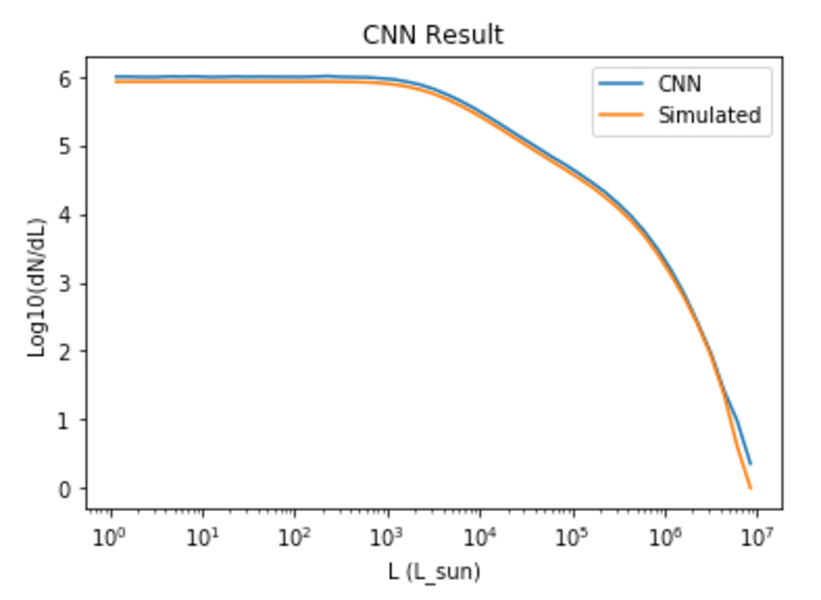
\includegraphics[width=0.8\textwidth]{CNN_4_layer_log.pdf}
				\caption{Plot showing the comparison of the output of the 4 layer CNN to the expected result of the underlying luminosity function that made the intensity map.}
				\label{fig:CNN_4_layer_log}
			\end{figure}

			\begin{figure}[H]
				\centering
				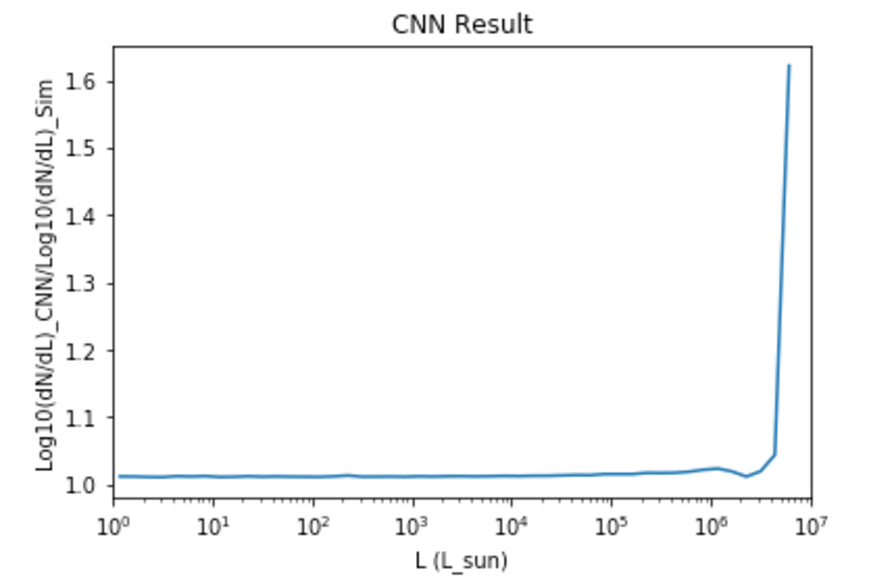
\includegraphics[width=0.8\textwidth]{CNN_4_layer_log_ratio.pdf}
				\caption{Plot showing the ratio of the CNN luminosity function over the underlying luminosity function.}
				\label{fig:CNN_4_layer_log_ratio}
			\end{figure}

			\begin{figure}[H]
				\centering
				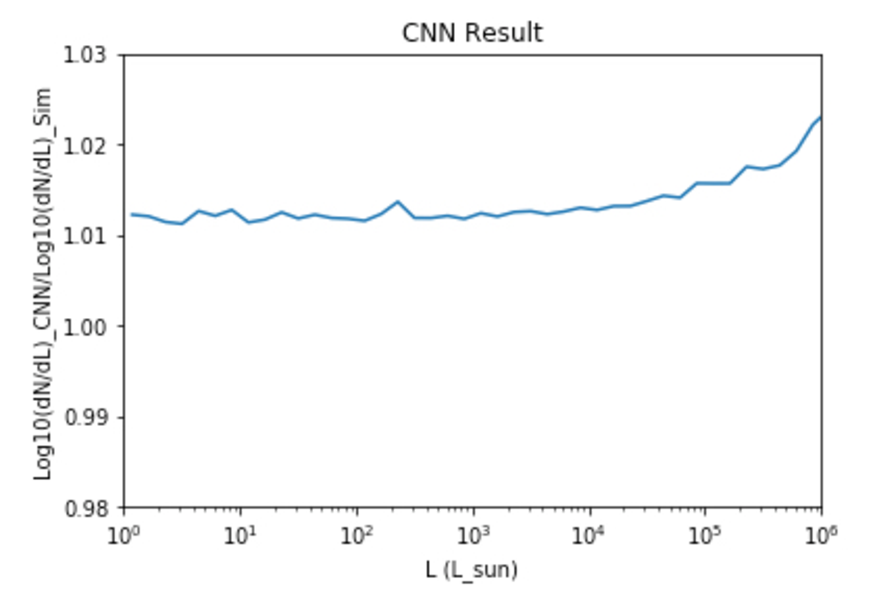
\includegraphics[width=0.8\textwidth]{CNN_4_layer_log_ratio_small.pdf}
				\caption{Zoom in of Figure \ref{fig:CNN_4_layer_log_ratio} showing the ratio of values before \(L = 10^6 L_{sun}\).}
				\label{fig:CNN_4_layer_log_ratio_small}
			\end{figure}

			We are probably interested in the actual values of things and not the log value so I checked the accuracy of the values instead of the log values.  The same set of plots but without logs are shown in \cref{fig:CNN_4_layer_log_unlog,fig:CNN_4_layer_log_unlog_ratio,fig:CNN_4_layer_log_unlog_ratio_small}.  What can be seen is that the error increases by at least an order of magnitude.  The error is still only around 20\%, but is still much larger then in the log case.  It can be shown (but I'm too lazy to type it out now) that the ratio of the unloged values is actually given by
			\begin{equation}
				\frac{dN}{dL}_{\rm{CNN}} / \frac{dN}{dL}_{\rm{sim}}(L) = 10^{\log \left(\frac{dN}{dL}_{\rm{sim}} (L)\right) * y(L)}
			\end{equation}
			where 
			\begin{equation}
				y = \log \left( \frac{dN}{dL}_{\rm{CNN}} \right) / \log \left( \frac{dN}{dL}_{\rm{sim}} \right)(L).
			\end{equation}

			\begin{figure}[H]
				\centering
				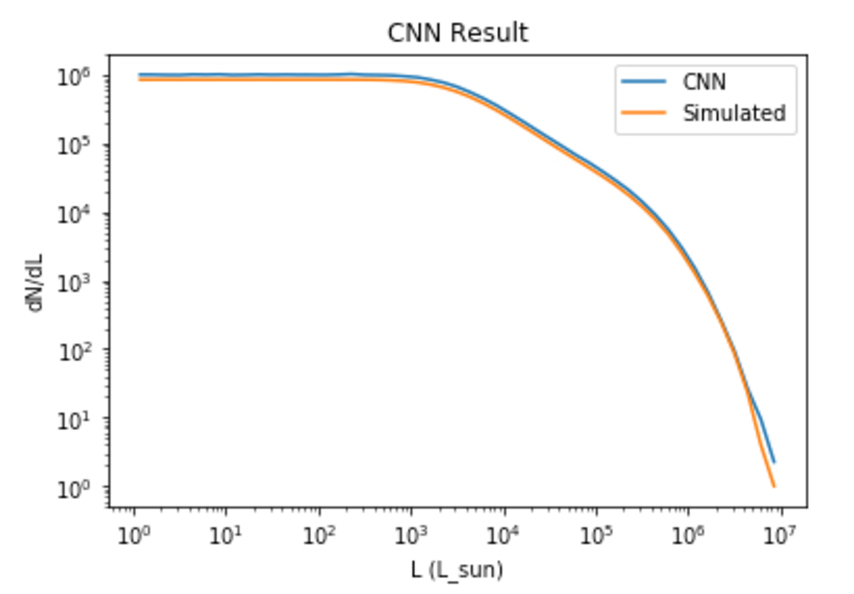
\includegraphics[width=0.8\textwidth]{CNN_4_layer_log_unlog.pdf}
				\caption{Plot showing the comparison of the output of the 4 layer CNN to the expected result of the underlying luminosity function that made the intensity map.}
				\label{fig:CNN_4_layer_log_unlog}
			\end{figure}

			\begin{figure}[H]
				\centering
				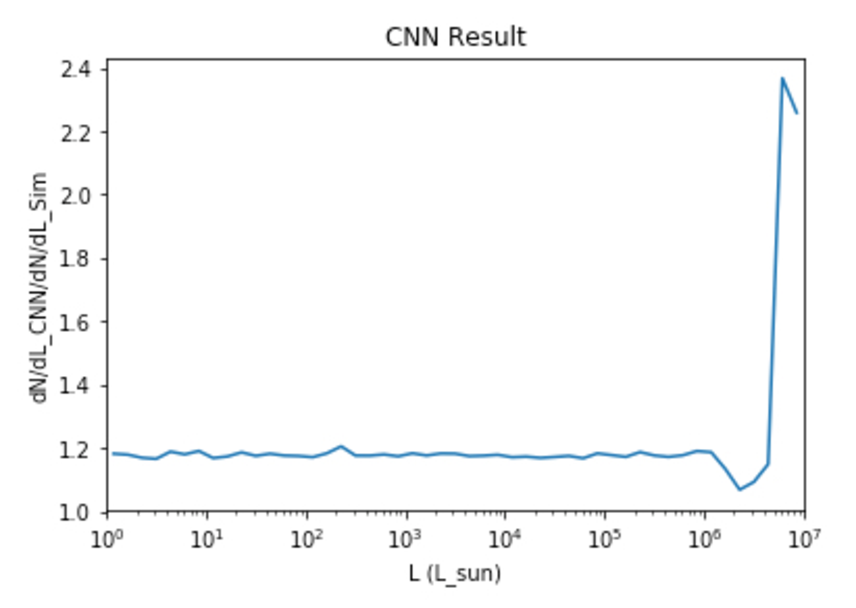
\includegraphics[width=0.8\textwidth]{CNN_4_layer_log_unlog_ratio.pdf}
				\caption{Plot showing the ratio of the CNN luminosity function over the underlying luminosity function.}
				\label{fig:CNN_4_layer_log_unlog_ratio}
			\end{figure}

			\begin{figure}[H]
				\centering
				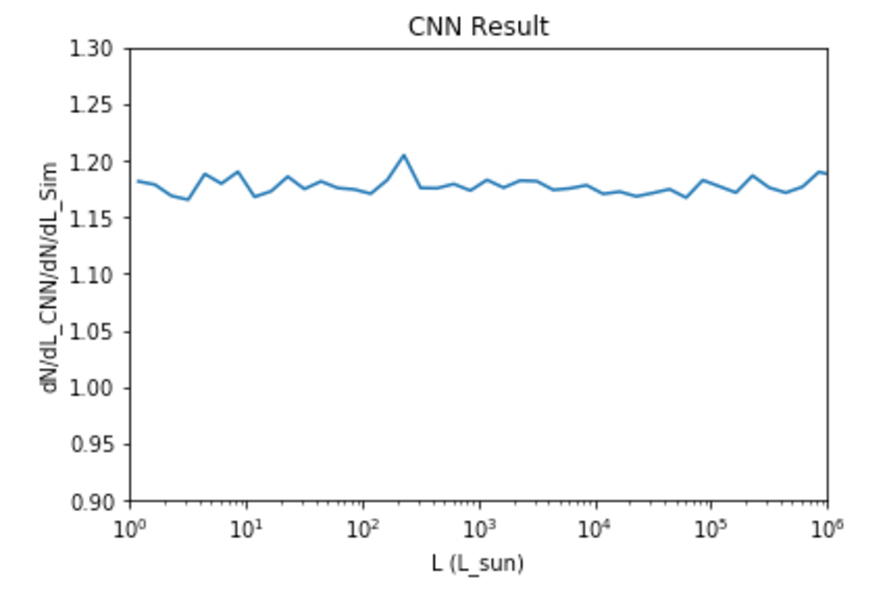
\includegraphics[width=0.8\textwidth]{CNN_4_layer_log_unlog_ratio_small.pdf}
				\caption{Zoom in of Figure \ref{fig:CNN_4_layer_log_ratio} showing the ratio of values before \(L = 10^6 L_{sun}\).}
				\label{fig:CNN_4_layer_log_unlog_ratio_small}
			\end{figure}

		\subsection{4 Layer dN/dL} \label{sec:4directValue}
			Seeing that finding the log luminosity value gives errors around 20\%, I tried to see if we could find the actual luminosity function directly.  The first network was 4 layers and was trained for 100 epochs of 400 maps apiece.  Each layer is a 3D convolution with kernel size 5 and stride 1 followed by a max pooling 3D of size 2 and stride 2.  The first layer has 32 filters, followed by 64, 128, 256 512.  Following the convolutional layers the network is flattened and then has a dense layer with 1000 neurons.  The final layer is another dense layer with a neuron for each point in the luminosity function we want.  Currently I take 50 points of the luminosity function.  The loss function was the mean log square error function.  Using mlse instead of mse makes it so that it doesn't get stuck trying to fit the region of low L and ignore the higher L regions where dN/dL is smaller. 

			I forget how long the network took to train, but it was under 48 hours.  Looking at \cref{fig:CNN_4_layer,fig:CNN_4_layer_ratio} one can see that the training did not go as well as it could.  There are discontinuities in the outputted luminosity function, sharp spikes and nothing after \(L \approx 10^6 L_{\rm{sun}}\).  I'm no expert, but we would want something better then that.  \cref{fig:CNN_4_layer_history_mlse,fig:CNN_4_layer_history_mse} show the training history of the loss function and another metric as a function of epoch while training 4 layer network.  The shape of \cref{fig:CNN_4_layer_history_mse} does look like what one would expect from a loss function.

			\begin{figure}[H]
				\centering
				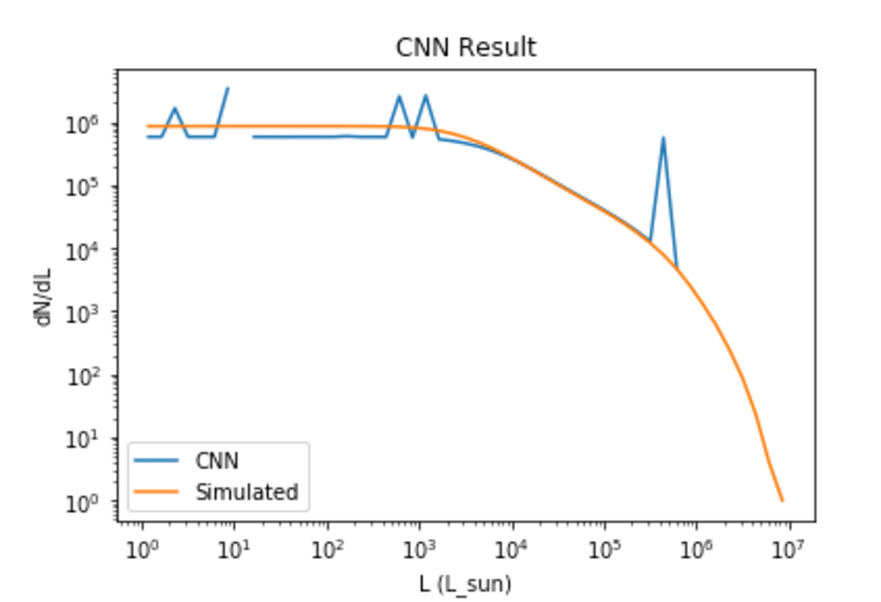
\includegraphics[width=0.8\textwidth]{CNN_4_layer.pdf}
				\caption{Plot showing the comparison of the output of the 4 layer CNN to the expected result of the underlying luminosity function that made the intensity map.}
				\label{fig:CNN_4_layer}
			\end{figure}

			\begin{figure}[H]
				\centering
				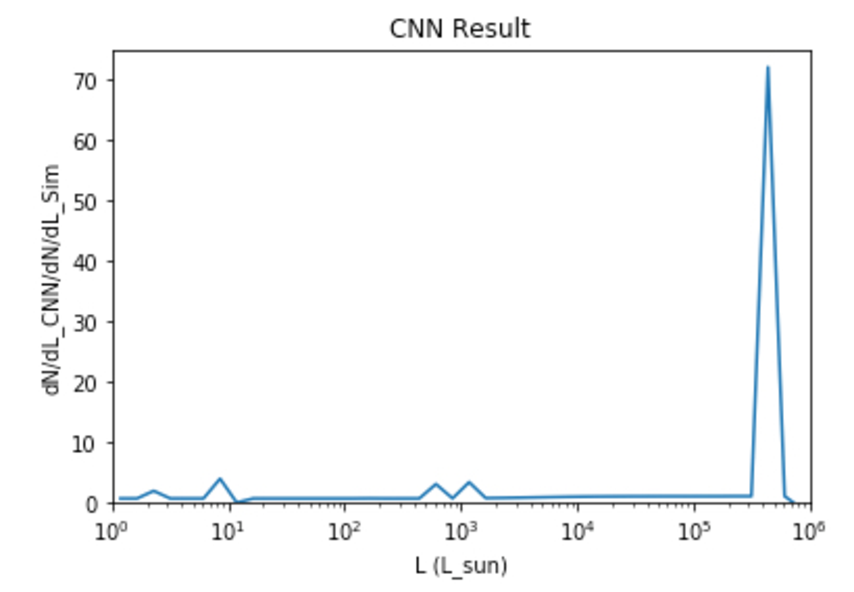
\includegraphics[width=0.8\textwidth]{CNN_4_layer_ratio.pdf}
				\caption{Plot showing the ratio of the CNN luminosity function over the underlying luminosity function.}
				\label{fig:CNN_4_layer_ratio}
			\end{figure}

			\begin{figure}[H]
				\centering
				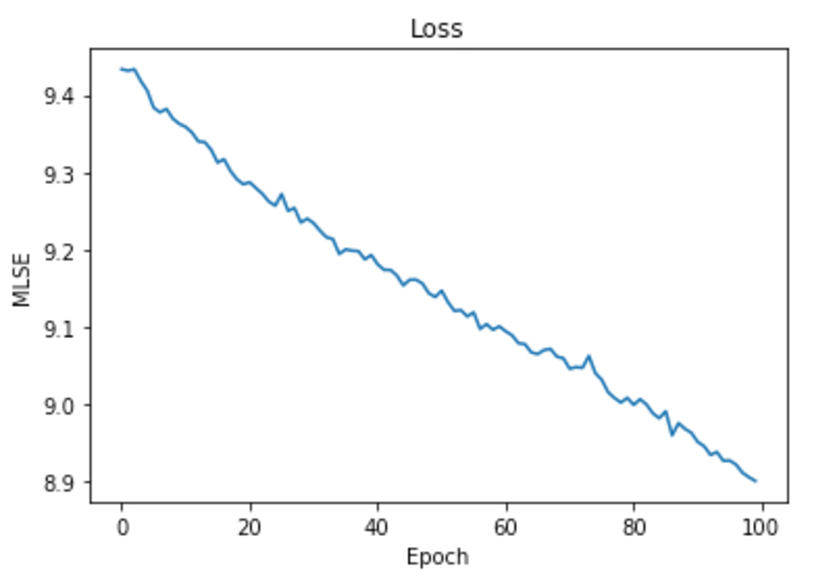
\includegraphics[width=0.8\textwidth]{CNN_4_layer_history_mlse.pdf}
				\caption{Plot showing loss history of the 4 layer CNN that was trained on the full luminosity function.  The loss function that was used was the mean log squared error}
				\label{fig:CNN_4_layer_history_mlse}
			\end{figure}

			\begin{figure}[H]
				\centering
				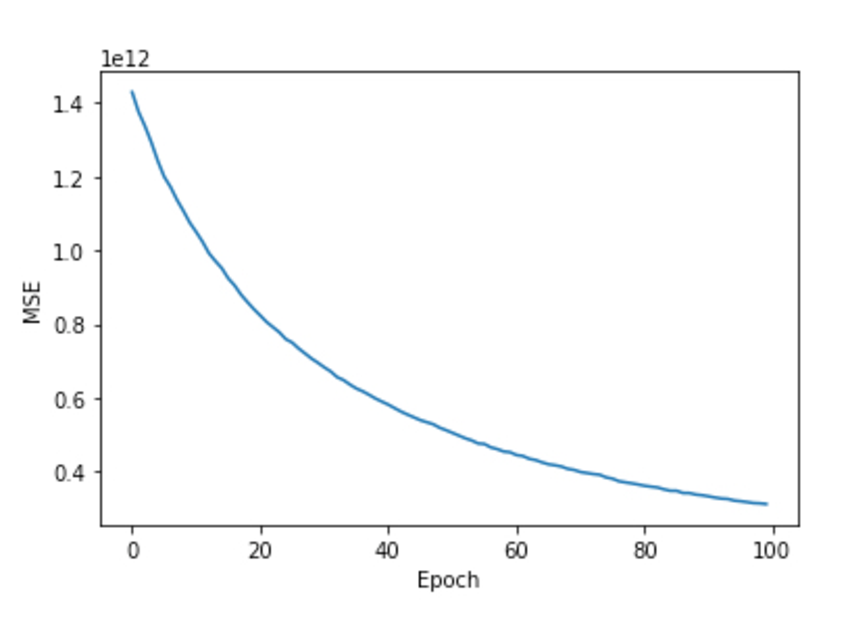
\includegraphics[width=0.8\textwidth]{CNN_4_layer_history_mse.pdf}
				\caption{Plot showing history of the mean squared error metric as a function of epoch.}
				\label{fig:CNN_4_layer_history_mse}
			\end{figure}

		\subsection{5 Layer dN/dL} \label{sec:5directValue}
			I tried making a 5 layer network, but it was much slower and only got around 30 epochs in 48 hours.  It was way too slow to train.  I saved every 20 epochs so not everything was wasted.  \cref{fig:CNN_5_layer} shows how "good" the semi-trained network is and it is pretty bad.  This needs more time.  I'm trying to run it for longer now and see if it will hopefully turn out better then the 4 layer network.

			\begin{figure}[H]
				\centering
				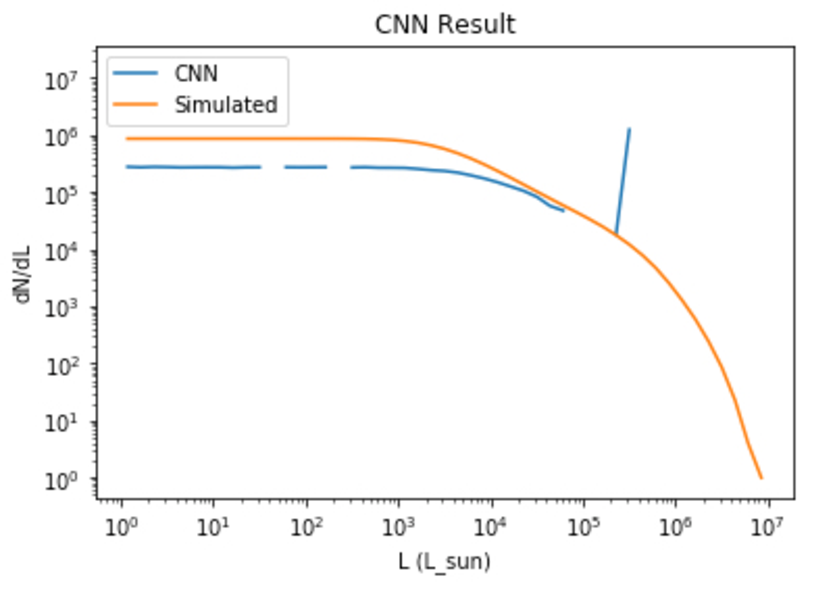
\includegraphics[width=0.8\textwidth]{CNN_5_layer.pdf}
				\caption{Plot showing the comparison of the output of the 5 layer CNN to the expected result of the underlying luminosity function that made the intensity map.}
				\label{fig:CNN_5_layer}
			\end{figure}



	\section{Things to do for Dan in no particular order}
		\begin{enumerate}
			\item Figure out what a good frequency bin size is

			\item \sout{Make maps and luminosity functions} Have done this for some maps and have the ability to do this for more

			\item \sout{Add in different halo luminosity relations to llm}

			\item \sout{Do some test runs with something basic}

			\item \sout{Make an actual CNN and try training it for an extended period of time}

			\item \sout{Get GPUs working correctly}

			\item \sout{Train on actual luminosity function instead of log(luminosity function)} Doesn't give the best results.  See Section \ref{sec:4directValue}.

			\item \sout{Get CNN to record loss and metric as it trains}

			\item Make lots of maps on MARCC to train with.  This will happen soon.
		\end{enumerate}


	
% \bibliography{draft}
\end{document}